\newcounter{ct}
\setcounter{ct}{1}
\whiledo{\value{ct} < 6}%
{%
  \ifnum \value{ct}=1
    \phantomsection\pdfbookmark[section]{Remerciements}{rem}
  \fi
  \begin{center}
  \includegraphics[width=0.9\linewidth,page=\thect]{Texte/Partie0/Preface/Remerciement.pdf}
  \end{center}
  \stepcounter{ct}%
}

\begin{comment}
%%%%%%% !!! Compile with XeLatex !!! //////////

%https://www.overleaf.com/project/5d95af765cb3ba00012a4ad5
\documentclass[12pt]{article}
\usepackage[paperheight=645pt, paperwidth=442pt, margin=0pt]{geometry}
\usepackage[french]{babel}
\pagestyle{empty}
\usepackage{fontspec}
\setmainfont{OpenDyslexicAlta}  %% uses a different "a"
\usepackage{setspace}
\usepackage{fmtcount}
\usepackage{tikzsymbols}
\begin{document}
\setstretch{1,5}
\textbf{\textit{\Large{Remerciements}}}

\vspace{.42cm}

Trente-et-un ans et presque autant d'années d'études, le périple fut long. Me voilà aujourd'hui Docteur, mais sans vous ce parcours n'aurait pu être. C'est l'occasion ici de vous remercier.\\

Déjà, remercier les membres de mon jury qui, avec enthousiasme et bienveillance, ont examiné mon travail et m'ont accordé ce titre. En particulier Pierre-Yves, mon directeur de thèse qui, dès ma première année de MASTER, a su me faire confiance et surtout me laisser toute la liberté dont j'avais besoin pour pouvoir m'exprimer et m'épanouir, alors pour ces 5 ans partagés avec toi et les membres de ton équipe, Merci. 

Chacun d'eux a su, tantôt me faire évoluer, tantôt me guider ; je pense notamment à Didier, sans qui rien n'aurait été possible.  Je pense également à toute l'équipe Poppy, Pierre, Matthieu, Nicolas, Damien et surtout Stéphanie et Théo qui ont été de vrais compagnons d'aventure pendant ces 3 années de thèse, et aujourd'hui des amis ; sans oublier Marie, aux prémices de l'aventure, 6 mois de stage laissent des souvenirs~\Winkey[0.6]~\dots~ Enfin, un petit clin d'oeil à l'ensemble des stagiaires que nous avons accueilli ; en particulier Tallulah pour son soutien, ses contributions, et sa compréhension durant cette dernière année qui n'a pas été la plus simple pour moi.

Mais bien sûr Flowers ne se résume pas à Poppy, et chacun a eu un rôle, alors Merci Alexendra, Fabien, Yoan, William, Benjamin, Sébastien, Baptiste, Thibaut, d'avoir été là et d'être comme vous êtes! Et, à tous ceux qui nous ont rejoint au fur et à mesure, je voudrais leur dire que je regrette de ne pas avoir eu plus le temps de vous découvrir, mais j'imagine que vous auriez été à la hauteur de vos prédécesseurs: exceptionnels.

Inria n'est pas qu'une équipe c'est une grande famille et je n'oublierai jamais cette ambiance cosmopolite, ces longues discussions autour d'un repas ou d'un café et surtout ces dizaines d'heures passées au Baby-Foot, cette soupape indispensable qui m'a permis de faire de grandes rencontres ; Merci, François, Brice, Manu, Philippe, Thibault, Grégoire et tous ceux dont je n'ai jamais su retenir les noms (foutu dyslexie) j'espère qu'ils se reconnaîtront (et qu'ils ne m'en voudront pas), Merci pour votre humour, votre ténacité, sans vous mes souvenirs d'Inria n'auraient pas la même saveur. 
Mais Inria ce n'est pas que des pauses, c'est aussi de nombreuses collaborations, notamment avec «~les filles de la com~» avec vous la vulgarisation scientifique est entre de bonnes mains! Merci à tous.

Évidemment, cette thèse aurait été incomplète sans toutes ces expériences réalisées, et je me dois de remercier tous ces enseignants qui ont accepté (sans forcement savoir exactement où ils mettaient les pieds) de jouer le jeu, ou plutôt d'avoir fait "jouer" leurs élèves avec mes robots! Ma plus grande fierté, c'est qu'ils continuent encore aujourd'hui, preuve que tout ceci aura eu un impact! Un Merci particulier à Joël qui, en toutes circonstances, a répondu présent à mes appels à l'aide lorsque je n'avais plus de sujet disponible ou un prototype à tester de toute urgence, Merci!

Je me dois également de remercier Anne, Laurent, Timothée, Estelle, Grégoire, Sébastien, Olivier et tous les autres membres du projet Perseverons, Merci pour votre appui, et surtout pour l'indépendance et l'autonomie que vous nous avez laissé pour conduire cette thèse.

Merci, à cette thèse de m'avoir permis tant de belles rencontres, Delphine, Marie-Aline, Thomas, Éric, Adrien, Sarah, Maud, je pense notamment à vous~\Winkey[0.6]

Merci, à mes p'tits robots d'avoir tenu le coup malgré tout ce que je vous ai fait endurer. Je crois qu'aujourd'hui je suis la personne qui vous connaît le mieux, j'espère qu'on ne vous oubliera pas!\\

Moi je n'oublie pas ceux qui m'ont permis d'en arriver jusqu'à cette thèse notamment Frédéric qui a fait le pari de me ré-intégrer dans le milieu universitaire après mes quelques années de tumulte. Je pense aussi à ceux qui m'ont donné l'envie d'enseigner, Marc-Michel, Glyn, Merci pour votre rigueur et votre désinvolture!\\

Merci à ceux qui m'ont permis d'enseigner, cela fut une vraie joie pour moi, que ce soit avec nos jeunes stagiaires de 3ème, ceux de MASTER2 ou mes élèves ingénieurs à L'ENSEIRB, ce fut un plaisir et j'ose croire que cela fut aussi enrichissant pour eux que pour moi.\\

J'aurai maintenant un Merci particulier à tous ceux qui, par le passé, n'auraient pas misé 10 Frs sur moi, vous m'avez donné la volonté et la persévérance pour vous prouver le contraire, voyez, malgré mon anti-conformisme, malgré ma dyslexie et tous les maux que vous avez pu me trouver, voyez, j'y suis arrivé!

Et bien sûr un immense Merci, à ceux qui ont cru en moi et vu le potentiel derrière l'ado à dompter. Merci Mme Séche, Merci Mr Ladureau, pour votre compréhension et l'exemple que vous avez su me donner. C'est peut-être déjà ici qu'est né mon amour d'apprendre, de comprendre et surtout d'expliquer pour que tous comprennent. Merci à vous, et à tous ceux pour qui le temps (et ma dyslexie) ne m'a pas permis de retenir vos noms\dots~ Karma vous le rendra~\Winkey[0.6]\\

Enfin, Merci à ceux qui m'accompagnent depuis mes premiers jours ; ma mère, pardon, ma Maman qui m'a soutenu contre vents et marrées, qui m'a pardonné un nombre incalculable de fois, qui m'a donné l'amour du débat, de l'amour tout court, qui est ce qu'elle est, avec ses qualités comme ses défauts \Tongey[0.6] et qui m'a permis de rendre ce travail sans trop de fautes, tu es sûrement l'une des 2 seules personne en ce monde à avoir lu chacun des mots de ce manuscrit avec toute la concentration que nécessite le déchiffrage de mon langage, Merci, sans toi je n'en serai pas là!

Merci Papa, tu es parti trop vite, je t'ai connu trop peu, mais l'impact ne se juge pas à la longueur, cet amour de la parole, ta volonté de changer le monde, à ton échelle, me guident encore chaque jour. J'espère que de là-haut tu es fier de moi, en tous cas je sais que tu n'as jamais douté!

Merci ma sœur, Caro, tu as joué de nombreux rôles, certains qui n'auraient pas dû t'être dévolus, mais tu l'as assumé, tu m'as toujours aidé, accompagné, envoyé chier, bref tu as toujours été là. Je ne sais pas si ça aurait pu être mieux, ou pire, mais je sais que je n'échangerai tout ça pour rien au monde, dans tes qualités et tes défauts tu m'as permis de grandir, mille Mercis, et pour l'anecdote, oui j'écris ces quelques mots à quelques heures de la deadline\dots~ comme toujours je gère l'urgence \Laughey[0.6] mais tu t'en doutais!

Guillaume, mon frère, qu'est ce que j'ai pu t'exaspérer, enfin d'apparence, haaa l'adolescence, quand j'entrais dans la mienne toi tu en sortais. Toi aussi tu as parfois dû jouer un rôle qui n'était pas le tiens et je rêve de pouvoir revenir à ma tendre enfance lorsque nous étions simples enfants, deux frères, une sœur et deux parents. Malgré tout, je ne changerai rien, même si je rêvais d'autre chose, cette coquille que tu arbores et que j'ai mis tant de temps à appréhender, à analyser, à comprendre, m'a donné le grain à moudre qui forgeât mon esprit. Aujourd'hui je sais que cette exaspération était emplie d'amour, et que ces petits noms dont tu m'affublais m'ont construit notamment le célèbre «la science» tout cela m'a conduit jusqu'ici, Merci à toi, pour tout! 

Une pensée pour le reste de ma (grande) famille qui, à mon goût, vivait trop loin, mais qui constitue les racines dont je tiens ma force. %\Wintertree[0.6]

Et bien sûr une pensée pour Annick, ma nourrice, ton naturel, ta bonté, ta naïveté m'ont donné cette petite chose en plus qui me fait croire et espérer, Merci.\\

Enfin, je dois maintenant remercier celle qui m'accompagne depuis 15 ans déjà, dans les hauts, dans les bas. Elle est celle qui à chaque instant a su me rappeler aux choses essentielles de la vie. L'amour, la haine, la vie, la mort, sans elle toutes ces choses auraient une autre saveur et je ne serais pas là. Merci de m'avoir aidé, accompagné, d'avoir grandi avec moi, cette thèse c'est aussi un peu la tienne, dans ses défauts comme dans ses qualités. Merci Léna, Merci d'être là, Merci pour ces deux merveilleux enfants que tu m'as donné. Merci Louka, Merci Eliot d'avoir supporté nos joies, nos peines, parfois mes absences, une thèse c'est chronophage, Merci Léna d'avoir toujours été là pour eux et pour moi. $\heartsuit$ Je vous aime! $\heartsuit$\\

Merci à mes amis passés, présents et à venir, Merci à tous ceux que j'oublie, les bons comme les mauvais, chacun d'eux a eu un rôle, qu'il en manque un et tout aurait été différent, alors MERCI! 

\begin{center}

\includegraphics[width=0.25\linewidth]{rond.png}
\end{center}

\end{document}
\end{comment}